\documentclass[a4paper,11pt]{article}
\usepackage{pdflscape}
\usepackage[utf8]{inputenc}
\usepackage[T1]{fontenc}
%\usepackage{fourier} % math & rm
%\usepackage{amsthm,amsfonts,amsmath,amssymb,textcomp}
\usepackage{pst-all,pstricks-add,pst-eucl}
\everymath{\displaystyle}
\usepackage{fp,ifthen}
%\usepackage{color}
%\usepackage{graphicx}
\usepackage{setspace}
\usepackage{array}
\usepackage{tabularx}
\usepackage{supertabular}
\usepackage{hhline}
\usepackage{variations}
\usepackage{enumerate}
\usepackage{pifont}
\usepackage{framed}
\usepackage[fleqn]{amsmath}
\usepackage{amssymb}
\usepackage[framed]{ntheorem}
\usepackage{multicol}
\usepackage{kpfonts}
\usepackage{manfnt}

%\usepackage[hmargin=2.5cm, vmargin=2.5cm]{geometry}
\usepackage{vmargin}          % Pour fixer les marges du document
\setmarginsrb
{1.5cm} 	%marge gauche
{0.5cm} 	  %marge en haut
{1.5cm}     %marge droite
{0.5cm}   %marge en bas
{1cm} 	%hauteur de l'entête
{0.5cm}   %distance entre l'entête et le texte
{1cm} 	  %hauteur du pied de page
{0.5cm}     %distance entre le texte et le pied de page

\newcommand{\R}{\mathbb{R}}
\newcommand{\N}{\mathbb{N}}
%\newcommand{\D}{\mathbb{D}}
\newcommand{\Z}{\mathbb{Z}}
\newcommand{\Q}{\mathbb{Q}}
\newcommand{\C}{\mathbb{C}}
\newcommand{\e}{\text{e}}
\newcommand{\dx}{\text{d}x}
\newcommand{\vect}[1]{\mathchoice%
  {\overrightarrow{\displaystyle\mathstrut#1\,\,}}%
  {\overrightarrow{\textstyle\mathstrut#1\,\,}}%
  {\overrightarrow{\scriptstyle\mathstrut#1\,\,}}%
  {\overrightarrow{\scriptscriptstyle\mathstrut#1\,\,}}}
\newcommand\arraybslash{\let\\\@arraycr}
\renewcommand{\theenumi}{\textbf{\arabic{enumi}}}
\renewcommand{\labelenumi}{\textbf{\theenumi.}}
\renewcommand{\theenumii}{\textbf{\alph{enumii}}}
\renewcommand{\labelenumii}{\textbf{\theenumii.}}
\renewcommand{\and}{\wedge}

\theoremstyle{break}
\theorembodyfont{\upshape}
\newcounter{enonce}
\newframedtheorem{theorem}[enonce]{Théorème}
\newframedtheorem{proposition}[enonce]{Proposition}
\newframedtheorem{definition}[enonce]{Définition}

\newtheorem{Term}{Terminologie}
\newtheorem{Rq}[enonce]{Remarque}
\newtheorem{exemple}[enonce]{Exemple}
\newtheorem{demonstration}[enonce]{Démonstration}
%\newtheorem{exo}{Exercice}

%\theorembodyfont{\small \sffamily}
%\newtheorem{sol}{solution}

\newenvironment{sol}% 
{\def\FrameCommand{\hspace{0.5cm} {\color{black} \vrule width 1pt} \hspace{-0.7cm}}%
  \framed {\advance\hsize-\width}
  \noindent \small \sffamily  %\underline{Solution :}%\\
}%
{\endframed}

\newrgbcolor{vert}{0 0.4 0}
\newrgbcolor{bistre}{1 .50 .30}
\setlength\tabcolsep{1mm}
\renewcommand\arraystretch{1.3}

\everymath{\displaystyle}
\hyphenpenalty 10000 %supprime toutes les césures
%\setcounter{secnumdepth}{0}
%\newcounter{saveenum}

\usepackage[frenchb]{babel}
%\usepackage{fancyhdr,lastpage}
%\usepackage{fancybox}

%\headheight 15.0 pt
%\fancyhead[L]{Leçon}
%\fancyhead[C]{}
%\fancyhead[R]{Chapitre 1}
%\fancyfoot[L]{{\scriptsize\textsl{Thomas Gire Cité scolaire de Lorgues}}}
%\fancyfoot[C]{\scriptsize\thepage}
%\fancyfoot[C]{\scriptsize\thepage/\pageref{LastPage}}

\title{Probabilités.}
\author{}
\date{}

%\pagestyle{empty}
%\pagestyle{fancy}
\usepackage[np]{numprint}

\renewcommand\arraystretch{1.8}

\newcounter{numero}
\newcommand{\exo}{
  \addtocounter{numero}{1}%
  \textbf{\underline{Exercice \arabic{numero}:}}\quad}

\frenchbsetup{StandardEnumerateEnv=true}
\usepackage{etex}
\usepackage{tikz,tkz-tab}
\usepackage{graphicx}
\graphicspath{ {../images/} }





\begin{document}
  %\setlength{\unitlength}{1mm}
  %\setlength\parindent{0mm}
 
  \maketitle


  
  \section{Définition.}
 
  \begin{definition}
  Une \textbf{probabilité} sur un univers fini 
  $\Omega=\lbrace \omega_1,...,\omega_n \rbrace$ est la donnée
  d'une fonction $$P:\Omega \to [0;1] \textrm{ telle que }
  \sum_{i=1}^n P(\omega_i)=1$$
  
  On appelle \textbf{éventualité} ou \textbf{issue} un élément 
  $\omega_i$ de $\Omega$.
  
  On appelle \textbf{événement} une partie $A$ de $\Omega$, i.e un ensemble d'issues.
  
  On peut étendre $P$ aux événements:
  $$
  \begin{array}{llll}
		P:&\mathcal{P}(\Omega) &\to& [0,1] \\
		  &A                   & \mapsto &
		  P(A)=\sum\limits_{\omega \in A} P(\omega)\\
  \end{array}
  $$
   
  \end{definition}
  
   Modéliser le caractère aléatoire d'une expérience consiste à définir une fonction de probabilité 
  sur l'ensemble des issues de cette expérience.
  
     \begin{exemple} 
   On réalise un lancer d'un dé équilibré à $6$ faces.
   
   Quelle est la probabilités d'obtenir un résultat pair ?
   
   $\Omega=\lbrace 1,..,6 \rbrace$, $A=
   \lbrace \omega \in \Omega / \omega \textrm{ est pair} \rbrace=
   \lbrace \omega
    \textrm{ est pair} \rbrace =\lbrace 2;4;6 \rbrace$.
    
    Le dé étant équilibré, il y a 
    équiprobabilité et $P(1)=P(2)=P(3)=P(4)=P(5)=P(6)=p$.
    
    Or $P(\Omega)=1=\sum\limits_{i=1}^6 P(i)=6 \times p$,
    
    donc $p=\frac{1}{6}$.
    
    Comme $P(A)=P(2)+P(4)+P(6)$,
    
    on a $P(A)=3 \times \frac{1}{6}=\frac{1}{2}$.
    
    De façon équivalente, comme il y a équiprobabilité, on peut écrire:
    
    $P(A)=\frac{Card(A)}{Card(\Omega)}=\frac{3}{6}=\frac{1}{2}$ où Card signifie le nombre d'éléments.

  \end{exemple}
  
  \newpage

    \section{Suites d'experiences aléatoires.} 
    

  \begin{theorem}
      Lorsqu'une expérience aléatoire (ou épreuve) est 
      constituée d'une suite de n expériences aléatoires, 
      on peut la représenter par un arbre pondéré. 
      Une issue est la liste ordonnée des résultats que l'on peut 
      représenter par un chemin de l'arbre.
      
      \begin{itemize}
      
      \item Loi des chemins:
       
       La probabilité d'une issue est le produit des 
       probabilités inscrites sur chacune des arêtes
       constituant le chemin associé à cette issue.
       
       \item Loi des noeuds:
       
       La somme des probabilités inscrites sur les arêtes
       issues d'un même noeud vaut 1.
       
       
      \end{itemize}

   \end{theorem}
   
      \begin{definition}
   On dit qu'une expérience aléatoire est constituée d'une suite d'épreuves \textbf{indépendantes},
   \textbf{identiquement distribuées} si chaque épreuve ne dépend pas des résultats des épreuves 
   précédentes, c'est à dire si les issues possibles sont les mêmes et avec la même répartition
   de probabilités.
  \end{definition}
 
 
  
    \begin{exemple}[Page 319]
   
   \begin{itemize}
    \item Tirage avec remise (épreuves indépendantes, identiquement distribuées)
    dans une urne contenant 2 boules bleues, 2 rouges et une noire.

  \item Représentation de l'expérience par un arbre pondéré.

   \end{itemize}
   \center{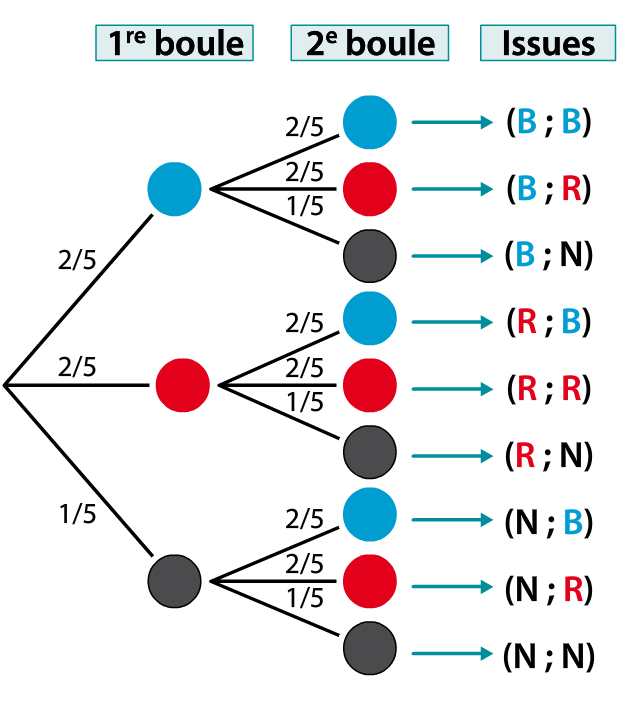
\includegraphics[scale=0.7]{../Images/issues.png}}
  \end{exemple}

 \section{Variables aléatoires.}
  
  \subsection{Définition.}
  
  
   \begin{definition}
      Etant donnée une expérience aléatoire dont l'univers (l'ensemble des issues possibles) est 
      $\Omega$. Définir une \textbf{variable aléatoire} (réélle) $X$ sur $\Omega$ consiste à associer à
      chaque issue un nombre réél. Autrement dit, $X$ est une fonction $X:\Omega \to \mathbb{R}$.
   \end{definition}
  
  
  
    \begin{exemple}
   
   On définit, sur l'expérience aléatoire de l'exemple précédent, la variable (aléatoire) qui
   associe à un tirage le nombre de boule rouge obtenue.
   
   Il n'y a que $3$ valeurs possibles pour cette variable aléatoire: $0,1,2$.
  
   \end{exemple}
  
  
  \subsection{Loi de probabilité.}
  
  
  \begin{definition} 
    
   Soit $\Omega$ un univers muni d'une fonction de probabilité $P:\Omega \to [0;1]$.
   
   Soit $X$ une variable aléatoire $X:\Omega \to \mathbb{R}$ avec $x_i,i=1,..,k$ ses différentes 
   valeurs.
   
   \'Etablir la \textbf{loi de probabilité} de $X$ consiste à associer à chaque valeur $x_i$ la probabilité
   de l'événement $X=x_i$.
   
   \end{definition}
   
    \begin{exemple}
    Soit $X$ la variable aléatoire qui compte le nombre de boules rouges tirées, de l'exemple précédent.

    \begin{multicols}{2} 
 
 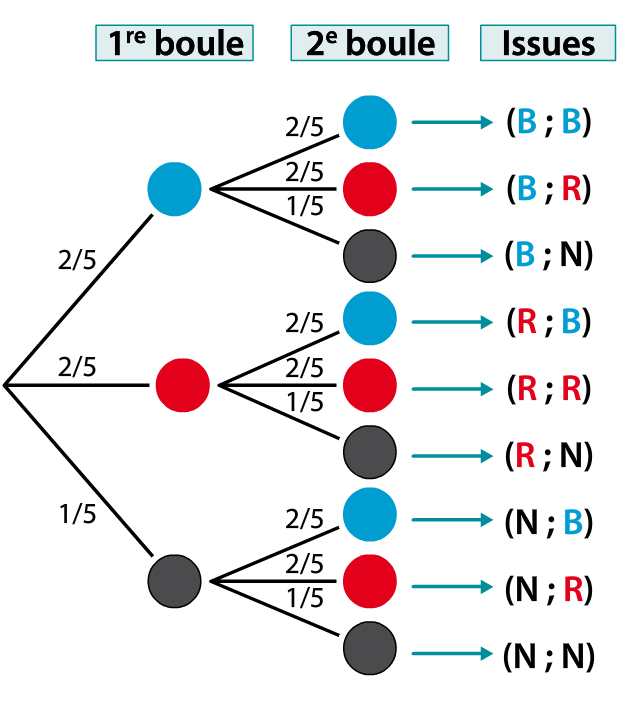
\includegraphics[scale=0.5]{../Images/issues.png}
 
 \renewcommand{\arraystretch}{2.2}
 $$
\begin{array}{|c|c|c|c|}

\hline
    x_i&0&1&2\\
    \hline
    P(X=x_i)&\frac{9}{25}&\frac{12}{25}&\frac{4}{25}\\
    \hline
    \end{array} 
$$  
 
\columnbreak 
 
 \small 
\begin{tabular}{ll}
    $P(X=0)$\\
    $=P(\lbrace(B;B);(B;N);(N;B);(N;N)\rbrace)$ \\
    $=P(B;B)+P(B;N)+P(N;B)+P(N;N)$\\
    $=(\frac{2}{5})^2+\frac{2}{5}\frac{1}{5}+\frac{1}{5}\frac{2}{5}+(\frac{1}{5})^2=\frac{9}{25}$\\
    \end{tabular}
    
\begin{tabular}{ll}
    $P(X=1)$\\
    $=P(\lbrace(B;R);(R;B);(R;N);(N;R)\rbrace)$ \\
    $=P(B;R)+P(R;B)+P(R;N)+P(N;R)$\\
    $=(\frac{2}{5})^2+(\frac{2}{5})^2+\frac{2}{5}\frac{1}{5}+\frac{1}{5}\frac{2}{5}=\frac{12}{25}$\\
    \end{tabular} 
    
\begin{tabular}{ll}
    $P(X=2)$\\
    $=P(\lbrace(R;R)\rbrace)$ \\
    $=P(R;R)$\\
    $=(\frac{2}{5})^2=\frac{4}{25}$\\
    \end{tabular} 


  
 
\end{multicols}
\end{exemple}

\subsection{Paramètres d'une variable aléatoire.}
               
Une loi de probabilité d'une variable aléatoire $X$:
 $$
\begin{array}{|c|c|c|c|c|}

\hline
    x_i&x_1&x_2&...&x_k\\
    \hline
    P(X=x_i)&p_1&p_2&...&p_k\\
    \hline
    \end{array} 
$$ 

est l'estimation des fréquences obtenues en faisant des statistiques sur un grand
nombre de réalisations de l'expérience aléatoire:
 $$
\begin{array}{|c|c|c|c|c|}

\hline
    x_i&x_1&x_2&...&x_k\\
    \hline
    f_i&f_1&f_2&...&f_k\\
    \hline
    \end{array} 
$$ 
 
De même que nous avons défini les paramètres moyenne, variance et écart-type d'une série statistique, 
nous définissons espérance $E(X)$, variance $var(X)$ et écart-type $\sigma_X$ d'une variable aléatoire $X$.

  \begin{definition}[Paramètres d'une variable aléatoire] 
    
   $$E(X)=\sum_{i=1}^k p_i x_i=p_1 x_1+...+p_k x_k$$
   
   $$Var(X)=E((X-E(X))^2)=\sum_{i=1}^k p_i (x_i-E(X))^2=E(X^2)-E(X)^2=\sum_{i=1}^k p_i x_i^2-(\sum_{i=1}^k p_i x_i)^2$$
   
   $$\sigma_X=\sqrt{Var(X)}$$
   \end{definition}
   
     \begin{exemple}
    
    On reprend l'exemple du tirage de boules de l'exemple précédent:
    
    $E(X)=0 \times P(X=0)+1 \times P(X=1)+2 \times P(X=2)$
    
    $=\frac{12}{25}+2 \times \frac{4}{25}=\frac{20}{25}
    =\frac{4}{5}$
    
    $E(X^2)=0^2 \times P(X=0)+1^2 \times P(X=1)+2^2 \times P(X=2)$
    
    $=\frac{12}{25}+4 \times \frac{4}{25}=\frac{28}{25}$
    
    $Var(X)=\frac{28}{25}-(\frac{20}{25})^2=\frac{28\times 25- 20 \times 20}{25^2}=\frac{300}{25^2}
    =\frac{3\times 4}{25}=\frac{12}{25}$
    
    $\sigma_X=\frac{2\sqrt{3}}{5}\simeq 0.69$
   \end{exemple}

     \begin{theorem}
    Soit $X:\Omega \to \mathbb{R}$ une variable aléatoire. On note $aX+b$ la variable aléatoire
     telle que $(aX+b)(\omega)=aX(\omega)+b$.
     
      \begin{centering}
      \begin{tabular}{c c}
   $E(aX+b)=aE(X)+b$,& $Var(aX+b)=a^2 var(X)$ 
   \end{tabular}

   \end{centering}
     
   \end{theorem}
   
      \begin{theorem}[Loi des grands nombres]
    
    Pour un grand nombre d'expériences aléatoires réalisées la moyenne (resp. l'écart-type)
    des valeurs observées pour $X$ est proche de l'espérance (resp. l'écart-type) de $X$.
    
   \end{theorem}
   
   \newpage
 
   
    \section{Schémas de Bernoulli.}
  \subsection{\'Epreuve de Bernoulli.}

  \begin{definition}[Schéma de Bernoulli d'ordre 1]
    Une \textbf{épreuve de Bernoulli} est une expérience aléatoire qui admet exactement deux issues:
    Succès et echec.
    
    En associant à cette expérience aléatoire la variable $X$ qui vaut $1$ en cas de succès et 
    $0$ en cas d'échec, on obtient pour X la loi de probabilité suivante:
     
     \renewcommand{\arraystretch}{1.5}
 $$
\begin{array}{|c|c|c|}

\hline
    k&0&1\\
    \hline
    P(X=k)&1-p&p\\
    \hline
    \end{array} 
$$   
     On dit que $X$ suit une \textbf{loi de bernoulli} de paramètre $p$ et on note $X \hookrightarrow B(p)$.
  \end{definition}

  
 
   \begin{exemple}
    On lance un dé équilibré à 6 faces. On définit le succès par l'événement <<Obtenir 6>>.
    La variable aléatoire associée à cette épreuve de Bernoulli suit la loi de Bernoulli
    de paramètre $\frac{1}{6}$.
    
    $X \hookrightarrow B(\frac{1}{6})$
    
    \renewcommand{\arraystretch}{2.2}
     $$
\begin{array}{|c|c|c|}

\hline
    k&0&1\\
    \hline
    P(X=k)&\frac{5}{6}&\frac{1}{6}\\
    \hline
    \end{array} 
$$
  
 \end{exemple}

  \begin{proposition}
  Soit $X$ une variable aléatoire suivant une loi de bernoulli de paramètre $p$.
  $$E(X)=p$$ $$Var(X)=p(1-p)$$
  
 \end{proposition}

  \begin{exemple}
 Dans la situation de l'exemple précédent:
 
 $E(X)=p=\frac{1}{6}$
 
 $Var(X)=\frac{1}{6} \times \frac{5}{6}=\frac{5}{36}$.
  
 \end{exemple}
 
 \newpage
 \subsection{Schéma de Bernouilli d'ordre n}

  
  \begin{definition}[Schéma de Bernoulli d'ordre $n$]
  On appelle \textbf{schéma de Bernoulli} d'ordre $n$ et de paramètre $p$, 
  l'expérience aléatoire constituée
  par une suite de $n$ épreuves de Bernoulli de pramètre $p$, indépendantes et identiquement distribuées.
  
  Le résultat de l'expérience est la liste des $n$ résultats représentée par un mot
  $$R_1R_2...R_n$$
  où $R_i= S$ ou $\overline{S}$.
  
  On peut représenter l'expérience par un arbre pondéré et la probabilité d'une issue est:
  $$p^k(1-p)^{n-k}$$ où $k$ est le nombre de succès.
 \end{definition}

 
   \begin{exemple}
 On réalise $3$ lancers successifs d'un dé équilibré, en considérant à chaque lancé <<obtenir 6>>
 comme le succès. La suite de ces trois épreuves de Bernoulli peut être représentée par l'arbre pondéré
 suivant:
 
  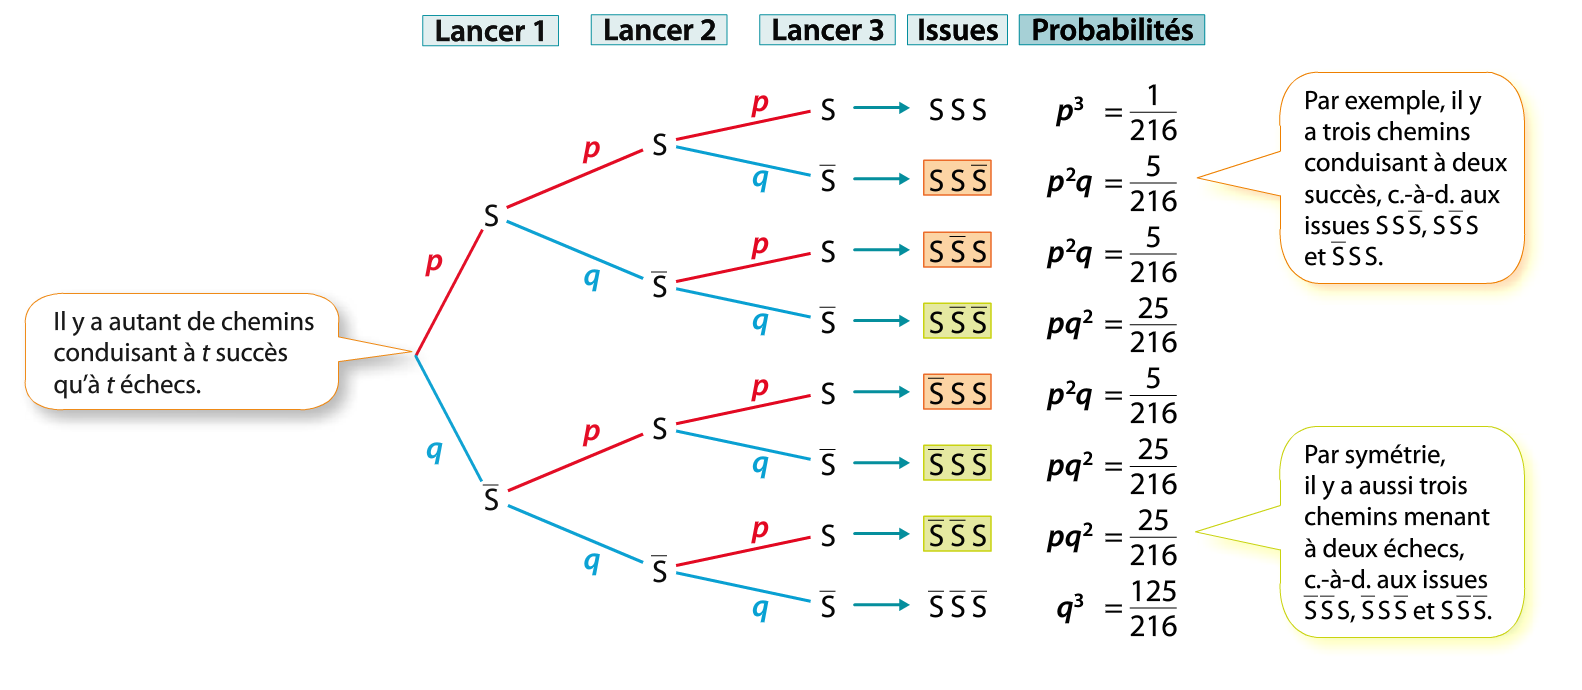
\includegraphics[scale=0.4]{../Images/arbreBinom.png}
 
  
 \end{exemple}
 
 \subsection{Loi binomiale.}

 
  
  \begin{definition}[Variable aléatoire associée]
  \`A un schéma de Bernoulli d'ordre $n$ et de paramètre $p$, on associe la variable aléatoire $Y$
  qui compte le nombre de succès obtenu lors de cette suite d'épreuves de bernoulli indépendantes et 
  identiquement distribuées. 
  
  Les valeurs possibles pour $Y$ sont $0,1,...,n$.
 \end{definition}
  On représente l'expérience par un arbre pondéré. L'évènement $\lbrace Y=k \rbrace$ est constitué 
  de tous les chemins de l'arbre contenant $k$ succès exactement. D'après la loi des chemins, la probabilité
  d'un tel chemin est $p^k(1-p)^{n-k}$. On appelle $C_n^k$ le nombre de tels chemins.


  \begin{theorem}
   On dit que la variable aléatoire $Y$ qui compte le nombre de succès lors d'un schéma de Bernoulli d'ordre $n$ et de paramètre $p$
   suit une \textbf{loi binomiale} de paramètres $n$ et $p$. On note $Y \hookrightarrow B(n,p)$.On a 
   \begin{centering}
      \begin{tabular}{c c c}
   $P(Y=k)=C_n^k p^k (1-p)^{n-k},$& $E(Y)=np,$ & $Var(Y)=np(1-p)$ 
   \end{tabular}

   \end{centering}

   
   
   
  \end{theorem}
  
  \subsection{Coefficients binomiaux.}


\begin{definition}
 On appelle coefficients binomiaux les entiers $C_n^k$ du théorème $21$.
 
 $C_n^k$ est le nombre de chemins empruntant exactement $k$ succès (et donc $n-k$ échecs),
 dans l'arbre binaire associé à un shéma de bernoulli d'ordre $n$.
 
 $C_n^k$ est aussi le nombre de façon d'écrire un mot de $n$ lettres composé de $k$ fois la 
 lettre $S$ et $n-k$ fois la lettre $E$.
 
 $C_n^k$ est aussi le nombre de parties à $k$ éléments d'un ensemble à $n$ éléments.
\end{definition}



 \begin{proposition}
  \begin{enumerate}
   \item $C_n^0=1$, pour tout entier naturel $n$.
   \item $C_n^k=C_n^{n-k}$, pour tout entier $n \geq 0$ et tout entier $0\leq k \leq n$. 
   \item Formule du \textbf{triangle de Pascal}:
   $$C_n^k=C_{n-1}^k+C_{n-1}^{k-1}$$ pour tout entier $n \geq 1$ et $1 \leq k \leq n$.
  \end{enumerate}

 \end{proposition}

 

 \begin{demonstration}
 
 \begin{enumerate}
   \item Il n'y a qu'un mot comportant que des échecs.
   \item D'après la symétrie de l'arbre.
   \item On distingue deux cas pour un chemin comportant exactement $k$
   succès: Soit il commence par un succès et il termine avec exactement $k-1$ succès durant les
   $n-1$ expériences restantes. Soit il commence par un échec et il termine avec exactement $k$ succès
   parmi les $n-1$ expériences restantes. 
  \end{enumerate}
  
 \end{demonstration}




   
   
\end{document}